\documentclass{report}

\usepackage{amsmath}
\usepackage{graphics}
\usepackage{textcomp}


%---Scale Command----%

\newcommand\scalemath[2]{\scalebox{#1}{\mbox{\ensuremath{\displaystyle #2}}}}

\input{preamble}
\input{macros}
\input{letterfonts}

\pagenumbering{arabic}

\title{\Huge{Controll Theory}\\Lecture 4}
\author{\huge{Jacek Grzegorzewski}}
\date{}

\begin{document}
\maketitle
\newpage% or \cleardoublepage
% \pdfbookmark[<level>]{<title>}{<dest>}
\pdfbookmark[section]{\contentsname}{toc}
\tableofcontents
\pagebreak

Now we concenrate or stationary systems, ie.
\begin{equation}
	\dot{x} = f(x)
\end{equation}
\dfn{Stationary systems}{
Stationary systems are systems independent of time, eg.
\begin{equation}
	\dot{x} = -2x(t) = f(x)
\end{equation}
As opposed to Nonstationary:
\begin{equation}
	\dot{x}(t) = 2 \sin(t)x(t) = f(x, t)
\end{equation}
}

$V(t,x) = V(x)$, and therefore it is always decresive(???)
Stability of $x_e$ is always uniform and t is the same in the case of asymptotic stability.

\dfn{Set invariant with respect to $\dot{x}=f(x)$}
{
	The set $\Omega \subset \mathbb{R}^{n}$ is invariant with respect to (1) iff $x_0 \in \Omega \rightarrow x(t,t_0,x_0) \in \Omega \forall t_0 t \geq t_0 $

}

\thm{}{Asume that there exist a solution of (1) for all $x_0 \in \Omega$. Suppose that there exist a function $V(x): \mathbb{R}^{n}  \longrightarrow R_T$ 
 such that: 
\begin{itemize} %% change to cases, so that it looks more like an equation
	\item $V$ is positive definite
	\item $V(x_e) = 0$
	\item V is radially unbounded
	\item $\frac{dV}{dx}$ exists and it is continuous on $\mathbb{R}^{n}$
\end{itemize}

\begin{itemize}
	\item $\dot{V} \leq 0$
	\item $\Omega = \{x_e\}$ is the only set that is invariant with respect to (1), amd
	\item $\Omega \subset \Omega_V = \{x \in \mathbb{R}^n I \dot{V}(x) = 0 \}$
\end{itemize}
Then the equalibrium point $x_e$ of (2) is  \textit{globally asymptoticaly stable}.
}

\ex{}{
	%$m\ddot{q} + k(q + q^3) + \alpha\dot{q} = 0$
\begin{itemize}
	\item $\dot{x_1} = x_2$	
	\item $\dot{x_2} = -\frac{k}{m}(x_1+x_1^3) - \frac{\alpha}{m}x_2$
\end{itemize}


\begin{equation}
	V(x) = 0.5m x_2 + k (0.5 x_1^2 + 0.2x_1^4)
	V(x_e=0) = 0
\end{equation}
}

\begin{equation}
	\dot{V(x(t,t_0))} = -\alpha x_2^2 \leq 0 %% xe is stable
\end{equation}


\chapter{Input / Output stability - introduction}


%% label this later as input output something, along edges
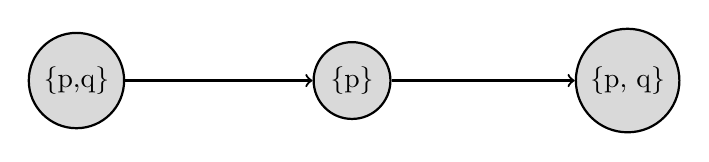
\begin{tikzpicture}[thick,node distance = {35mm},  main/.style = {draw, circle}]
	\node[main, fill = gray!30](1) {\{p,q\}};
	\node[main, fill = gray!30] (2) [right of=1] {\{p\}};
	\node[main, fill = gray!30] (3) [ right of=2] {\{p, q\}};
	\draw[->] (1) to [out=0, in=180, looseness=0.1] (2);
	\draw[->] (2) to [out=0, in=180, looseness=0.1] (3);
	
	%\caption{Input output equation}
\end{tikzpicture}

\nt{
\begin{itemize}
	\item Signal spaces - normed
	\item system spaces - normed operators associated with systems
\end{itemize}
}
\dfn{Normed linear space}
{
	Let $X$ be a linear space over  $\mathbb{R}$ or $\mathbb{C}$. A real valued function $\norm{x}$ defined on $X$ is said to be a norm if it satisfies the following properties:
	 \begin{enumerate}
		 \item $\norm{x} \geq 0  \forall x \in X $ (nonnegative)
		 \item $\norm{x} = 0 iff x = 0$(positive definite)
		 \item $\norm{\lambda x} = \norm{\lambda} \norm{x} \forall \lambda \in \mathbb{R} \forall x \in X $ (Linearity)
		 \item $\norm{ x + y} = \norm{x} \norm{y} \forall x,y \in X (Triangle inequality)$
	\end{enumerate} 
The Pair $(X, \norm{.})$ is said to be a normed linear space
}

\ex{Example norms}{
	\begin{itemize}
	%y = \Phi(\Sigma_{i = 0}^n{\omega_i v_i}+b)
		\item $\norm{x}_2 = \sqrt{\Sigma_{i = 1}^{n} \abs{x_i}^2}$
		\item $\norm{x}_1 = \Sigma_{i = 1}^{n} \abs{x_i}$
		\item $\norm{x}_{\inf} = \max_{i}\abs{x_i}$
	\end{itemize}
	}

\dfn{P-norm of a signal}
{
Consider $ 1 \leq p \leq \inf$. Let $x: \mathbb{I} \longrightarrow \mathbb{R}^n(\mathbb{C}^n)$, where $\mathbb{I}\subset \mathbb{R}$. The p--norm of x is defined a follows:
\begin{equation}
\norm{x}_p = (\int_{\mathbb{I}} (\norm(x(t)i)_K)^{p}dt)^{\frac{1}{p}} \forall 1 \le p < \inf
	\sup_{t \in \mathbb{I}} \norm{x(t)}_K \forall p = \inf 
\end{equation}
where $K \in \mathbb{N}$
}

\ex{Example of a P-norm}
{
\begin{itemize}
\item $g_1(t) = e^{-t}\cos(t)$
\item $g_2(t) = \overline{v} , t \in \mathbb{I} =\mathbb{R}_+\cup\{0\}$ %% change this vec to column vector
\end{itemize}
}

\dfn{$\mathcal{L}_p$ spaces}
{
$\mathcal{L}_p(\mathbb{I})$ space consist of $\mathbb{C}^{n}(\mathbb{R}^{n})$ valued functions $x(t)$ defined on $\mathbb{I} \subset \mathbb{R}$ such that $\norm(x)_p \le \inf$ with  $ 1 \le p \le \inf$.
}






\end{document}
